\chapter{Validation Fonctionnelle, Restitution et Évaluation}

Ce chapitre constitue le prolongement opérationnel des trois chapitres précédents. Nous y démontrons que l'architecture modulaire définie au Chapitre~I, les choix technologiques justifiés au Chapitre~II et les pipelines d'acquisition, de transformation et d'intelligence sémantique implémentés au Chapitre~III convergent vers un système fonctionnel, cohérent et directement utilisable par un analyste en renseignement sur les menaces. Nous procédons en deux temps. Dans un premier temps, nous validons la plateforme par la restitution visuelle : l'interface utilisateur et le tableau de bord central sont présentés comme surface de preuve de l'intégralité de la chaîne de traitement, depuis l'ingestion des indicateurs de compromission jusqu'à leur agrégation en temps réel. Dans un second temps, nous évaluons les performances du système par des tests de charge et des métriques quantitatives portant sur la latence de bout en bout, le débit d'ingestion et la capacité de corrélation sémantique du pipeline RAG. L'ensemble de cette validation est conduit sur l'instance de production déployée en local, sans données synthétiques ni simulateurs : chaque métrique et chaque capture d'écran présentées dans ce chapitre reflètent le comportement réel de la plateforme opérant sur des flux OSINT authentiques.

%% =========================================================================
\section{Interface Utilisateur et Tableau de Bord Central}
%% =========================================================================

L'interface utilisateur constitue la couche de restitution de la plateforme ONYX. Elle ne se limite pas à une fonction d'affichage passif : elle opère comme un système réactif de supervision en temps réel, capable de refléter l'état du pipeline d'acquisition avec une latence inférieure à 50~millisecondes entre l'événement serveur et sa projection visuelle dans le navigateur. Nous présentons ici l'architecture frontend, la gestion de l'état applicatif, le protocole de communication bidirectionnelle par WebSocket et leur intégration dans le tableau de bord central.

\subsection{Architecture Frontend : Next.js, React et Rendu Hybride}

Comme justifié au Chapitre~II (section~II.4), le tableau de bord repose sur le cadriciel Next.js~14 couplé à la bibliothèque React~18. L'architecture d'exécution adopte un modèle de rendu hybride qui sépare strictement les responsabilités entre serveur et client.

Le point d'entrée de la page principale (\texttt{src/app/page.tsx}) est un composant serveur (\textit{Server Component}) au sens de l'architecture React Server Components (RSC). Ce composant génère le balisage HTML initial côté serveur --- métadonnées SEO, balises de préchargement des polices, structure sémantique --- puis délègue l'intégralité de la logique interactive à un composant client chargé dynamiquement via la primitive \texttt{next/dynamic} avec l'option \texttt{ssr:~false}. Cette désactivation explicite du rendu côté serveur pour le composant de tableau de bord est une décision d'ingénierie motivée par deux contraintes techniques : premièrement, les bibliothèques de visualisation 3D (rendu WebGL de la carte de menaces géopolitiques) et les connexions WebSocket nécessitent l'API DOM du navigateur, absente dans l'environnement Node.js du serveur ; deuxièmement, le composant principal (\texttt{DashboardClient}) instancie au montage les connecteurs OSINT temps réel et les \textit{sockets} bidirectionnels, opérations qui ne doivent s'exécuter qu'une seule fois dans le cycle de vie du client.

Le composant \texttt{DashboardClient} orchestre une navigation par onglets entre neuf vues fonctionnelles : le \textit{Tableau de Bord Exécutif} (vue synthétique pour décideurs), la \textit{Vue Opérationnelle} (carte de menaces 3D, extracteur NLP SciBERT, flux SIEM), le \textit{Laboratoire IA} (pipeline RAG et assistant conversationnel Gemini), la \textit{Télémétrie IOC} (explorateur d'indicateurs de compromission et CVE actives), les \textit{Acteurs de Menace} (fiches détaillées APT avec TTPs MITRE associés), le \textit{Graphe de Menace} (visualisation topologique des relations inter-entités), le panneau \textit{Crawlers} (journaux d'acquisition temps réel sur Tor et Web de surface), le \textit{Générateur de Rapports} et la \textit{Matrice ATT\&CK} (couverture technique par catégorie tactique).

\subsection{Gestion de l'État Applicatif : Architecture Multi-Stores Zustand}

La gestion de l'état client constitue un défi architectural majeur pour une plateforme de supervision en temps réel. Les solutions classiques (Redux, Context API) présentent des limitations qui les rendent inadaptées à notre cas d'usage. Redux impose un modèle de flux de données unidirectionnel avec des \textit{reducers} immuables dont la sérialisation/désérialisation sur chaque mise à jour dégrade les performances lorsque le rythme de mise à jour atteint plusieurs dizaines d'événements par seconde. L'API Context de React, quant à elle, déclenche un re-rendu de l'ensemble des composants consommateurs à chaque modification de l'état, indépendamment de la granularité de la mutation, produisant un goulot d'étranglement sur le fil de rendu principal.

Nous avons retenu Zustand, une bibliothèque de gestion d'état qui résout ces deux problèmes par son modèle de souscription sélective. Chaque composant consommateur s'abonne explicitement au sous-ensemble de l'état dont il dépend via une fonction de sélection (\textit{selector}). Les mutations qui n'affectent pas les champs sélectionnés ne déclenchent aucun re-rendu du composant, offrant une complexité de mise à jour en $\mathcal{O}(1)$ par rapport au nombre total de champs de l'état global.

Notre architecture déploie cinq \textit{stores} Zustand spécialisés, chacun isolant un domaine fonctionnel distinct :

\begin{enumerate}
    \item \textbf{\texttt{useOnyxStore}} (store principal) : maintient l'état du canal WebSocket (indicateur de connexion, compteur de messages reçus, horodatage de fraîcheur), la liste des IOC armés, le flux d'événements temps réel (limité aux 150 derniers pour éviter la saturation mémoire), et les compteurs de session (nombre de reconnexions, nombre total d'IOC ingérés en direct). Ce store implémente également les actions de connexion/déconnexion WebSocket et le mécanisme de pause/reprise du flux avec tampon d'accumulation.
    \item \textbf{\texttt{useOmegaStore}} : encapsule l'état du module Omega (moteur de détection, analyse NLP par SciBERT, visualisation du graphe de menace, génération de bundles STIX~2.1). Ce store utilise l'intergiciel \texttt{subscribeWithSelector} de Zustand pour permettre aux composants de visualisation de réagir sélectivement aux mutations de sous-arbres spécifiques de l'état.
    \item \textbf{\texttt{useThemeStore}} : persiste le thème visuel (sombre ou clair) via l'intergiciel \texttt{persist} de Zustand, qui sérialise l'état dans le \texttt{localStorage} du navigateur. La fonction \texttt{applyPersistedTheme()} assure la synchronisation du thème entre le rendu côté serveur et l'hydratation côté client, évitant le phénomène de \textit{flash of incorrect theme} lors du chargement initial.
    \item \textbf{\texttt{useUserProfile}} : persiste le rôle de l'utilisateur (\texttt{EXPERT} ou \texttt{DECIDEUR}) pour adapter le niveau de détail technique de l'interface selon le profil. Cette ségrégation par profil implémente le principe de divulgation progressive (\textit{progressive disclosure}) de la norme ISO~9241-110.
    \item \textbf{\texttt{useActorDetailStore}} : maintient l'état de sélection inter-panneaux pour la vue de détail des acteurs de menace (nœud sélectionné dans le graphe, techniques MITRE surlignées, niveau de densité informationnelle de l'affichage progressif).
\end{enumerate}

\subsection{Communication Bidirectionnelle : Protocole WebSocket et Bus d'Événements}

\subsubsection{Justification du protocole WebSocket face aux alternatives}

Le rafraîchissement des données de supervision en temps réel peut être assuré par trois mécanismes : l'interrogation périodique (\textit{polling}), les événements poussés par le serveur (\textit{Server-Sent Events}, SSE) ou les WebSockets. Nous avons implémenté un modèle hybride qui exploite les trois mécanismes selon leurs forces respectives, mais dont le canal principal repose sur les WebSockets pour les raisons suivantes.

L'interrogation périodique (\texttt{setInterval} + \texttt{fetch}) impose une latence incompressible égale à la moitié de l'intervalle d'interrogation : pour un intervalle de 15~secondes, un événement survenant immédiatement après la dernière requête n'est détecté qu'après 15~secondes. De surcroît, chaque cycle d'interrogation génère une requête HTTP complète (en-têtes TCP, négociation TLS, en-têtes HTTP, sérialisation JSON), soit un surcoût protocolaire de l'ordre de 800 octets par requête même lorsqu'aucune donnée nouvelle n'est disponible. Pour une plateforme CTI recevant en moyenne 50 événements par minute, cette approche gaspille systématiquement la bande passante et la capacité de traitement du serveur.

Les Server-Sent Events (SSE) résolvent partiellement le problème de la latence en établissant un flux HTTP persistant unidirectionnel du serveur vers le client. Cependant, le protocole SSE est limité à une communication monodirectionnelle : le client ne peut envoyer de messages au serveur sans établir une connexion HTTP distincte. Cette limitation interdit l'implémentation de fonctionnalités telles que les battements de cœur bidirectionnels (\textit{ping/pong}), les abonnements dynamiques à des canaux spécifiques ou les accusés de réception d'événements. Nous conservons néanmoins les SSE pour le flux de journaux des crawlers, dont le modèle de communication est intrinsèquement unidirectionnel (le serveur émet les lignes de journal, le client ne fait que les afficher).

Le protocole WebSocket (RFC~6455), en revanche, établit un canal de communication bidirectionnel en duplex intégral sur une connexion TCP unique. Après la phase initiale de poignée de main HTTP (\textit{HTTP Upgrade handshake}), les trames WebSocket sont échangées avec un surcoût protocolaire de seulement 2 à 14 octets par trame, soit une réduction de deux ordres de grandeur par rapport au surcoût HTTP. Ce protocole constitue donc le vecteur optimal pour la diffusion d'alertes CTI où la latence de bout en bout doit demeurer inférieure au seuil perceptif humain de 100~millisecondes.

\subsubsection{Implémentation côté serveur : Hub WebSocket avec fan-out Redis}

Côté serveur, le point d'accès WebSocket est exposé sur le chemin \texttt{/ws/events} par le routeur FastAPI. L'architecture repose sur un gestionnaire de connexions singleton (\texttt{WSConnectionManager}) qui maintient un registre des connexions actives pour le processus courant et implémente trois mécanismes de sécurité :

\begin{itemize}
    \item \textbf{Validation d'origine (protection CSWSH)} : en mode production, l'en-tête \texttt{Origin} de chaque requête de connexion est vérifié contre la liste des origines autorisées dans la configuration CORS, empêchant les attaques par détournement de WebSocket inter-sites (\textit{Cross-Site WebSocket Hijacking}).
    \item \textbf{Limitation de débit par adresse IP} : un compteur par adresse IP limite le nombre de connexions simultanées à 10 par client, neutralisant les tentatives de saturation du serveur par épuisement de descripteurs de fichiers.
    \item \textbf{Authentification JWT} : en mode production, un jeton JWT valide est exigé comme paramètre de requête (\texttt{?token=<jwt>}) lors de la poignée de main. En mode développement, cette authentification est contournée pour faciliter le prototypage rapide.
\end{itemize}

La distribution des événements vers les clients repose sur le mécanisme de publication/abonnement (\textit{Pub/Sub}) de Redis. Chaque processus API exécute une tâche asynchrone dédiée (\texttt{\_redis\_listener}) qui s'abonne au canal Redis \texttt{onyx:ws:broadcast}. Lorsqu'un événement est publié sur ce canal --- par le poller OSINT, l'ingesteur géopolitique ou le moteur NLP --- il est automatiquement relayé à toutes les connexions WebSocket locales via la méthode \texttt{broadcast()} du gestionnaire. Ce modèle de fan-out par Redis garantit que les événements sont distribués uniformément à tous les clients, indépendamment du processus API qui a traité la requête initiale d'ingestion. Chaque trame émise est enveloppée dans un protocole JSON normalisé comportant quatre champs : le canal sémantique (\texttt{channel}), la charge utile (\texttt{payload}), l'horodatage ISO~8601 (\texttt{ts}) et un numéro de séquence monotone (\texttt{seq}) permettant au client de détecter les pertes de trames et de maintenir l'ordonnancement causal des événements.

\subsubsection{Implémentation côté client : Store réactif avec reconnexion exponentielle}

Côté client, la connexion WebSocket est intégrée directement dans le store Zustand principal (\texttt{useOnyxStore}). Ce choix architectural --- encapsuler la logique réseau dans le store plutôt que dans un hook React dédié --- présente un avantage déterminant : l'instance WebSocket est maintenue au niveau modulaire (variable \texttt{wsInstance} en portée de module), et non dans l'état local d'un composant. Cette séparation empêche le mode strict de React 18 (\textit{StrictMode}), qui monte et démonte les composants deux fois en développement, de créer des connexions WebSocket dupliquées et des fuites de ressources.

Le code suivant présente l'implémentation complète du moteur WebSocket intégré au store Zustand, incluant la connexion, la réception sécurisée des messages, la reconnexion à recouvrement exponentiel et le mécanisme de battement de cœur :

\begin{lstlisting}[language=JavaScript, caption={Moteur WebSocket intégré au store Zustand : connexion, sanitisation DOMPurify, \textit{batching} par \texttt{requestAnimationFrame} et reconnexion exponentielle.}, label={lst:ws-store}]
// --- Variables de module (hors composant React) ---
let wsInstance: WebSocket | null = null;
let reconnectTimer: ReturnType<typeof setTimeout> | null;
let reconnectDelay = 1000;  // Backoff exponentiel initial
let pingIntervalId: ReturnType<typeof setInterval> | null;

// --- Action connectWebSocket() dans le store ---
connectWebSocket: () => {
  // Garde : empeche les connexions dupliquees
  if (wsInstance) return;
  if (reconnectTimer) clearTimeout(reconnectTimer);

  // Construction dynamique de l'URL WebSocket
  const API = process.env.NEXT_PUBLIC_API_URL
            || 'http://localhost:8000';
  const wsUrl = API.replace(/^http/, 'ws')
              + '/ws/events';

  wsInstance = new WebSocket(wsUrl);

  wsInstance.onopen = () => {
    set({ connected: true });
    reconnectDelay = 1000; // Reset du backoff
    // Heartbeat toutes les 15s
    pingIntervalId = setInterval(() => {
      if (wsInstance?.readyState === WebSocket.OPEN)
        wsInstance.send(JSON.stringify({type:'ping'}));
    }, 15000);
  };

  wsInstance.onmessage = (event) => {
    // Phase 1: Parse + sanitisation DOMPurify
    const rawMsg = JSON.parse(event.data);
    const msg = sanitizePayload(rawMsg);

    // Phase 2: Tracking de fraicheur (Trust UX)
    set(s => ({
      lastWsMessageAt: Date.now(),
      wsMessageCount: s.wsMessageCount + 1,
    }));

    // Phase 3: Filtrage des trames de controle
    if (msg.channel === 'heartbeat'
     || msg.payload?.type === 'pong') return;

    // Phase 4: Construction de l'evenement
    const evt: WSEvent = {
      type: msg.channel || msg.payload?.type,
      data: msg.payload || {},
      timestamp: msg.ts || new Date().toISOString(),
    };

    // Phase 5: Pause/Resume avec tampon
    if (get().isFeedPaused) {
      set(s => ({
        feedBuffer: [...s.feedBuffer, evt]
                    .slice(-500)
      }));
      return;
    }

    // Phase 6: Accumulation + requestAnimationFrame
    eventQueue.push(evt);
    if (evt.type === 'ioc_detected' && evt.data)
      iocQueue.push(evt.data as IOC);
    scheduleBatch(); // processBatch() via rAF
  };

  // Reconnexion a recouvrement exponentiel
  // Delai: 1s -> 2s -> 4s -> 8s (plafond)
  wsInstance.onclose = () => {
    set(s => ({
      connected: false,
      reconnectCount: s.reconnectCount + 1,
    }));
    wsInstance = null;
    reconnectTimer = setTimeout(() => {
      reconnectDelay = Math.min(
        reconnectDelay * 2, 8000
      );
      get().connectWebSocket();
    }, reconnectDelay);
  };
},
\end{lstlisting}

Nous soulignons plusieurs aspects d'ingénierie critiques dans cette implémentation.

\textbf{Sanitisation systématique (DOMPurify).} Chaque message WebSocket entrant est soumis à la fonction \texttt{sanitizePayload()} avant toute exploitation. Cette fonction applique récursivement la bibliothèque DOMPurify sur les champs de type chaîne de caractères de la charge utile, neutralisant les vecteurs d'injection XSS (\textit{Cross-Site Scripting}) qu'un flux OSINT compromis pourrait véhiculer. Cette précaution est essentielle dans le contexte CTI : les données ingérées proviennent de sources potentiellement adverses (forums du Dark Web, blogs de rançongiciels), et un indicateur de compromission malicieusement formaté pourrait contenir du code JavaScript exécutable si injecté sans sanitisation dans le DOM.

\textbf{Agrégation par \texttt{requestAnimationFrame} (\textit{batching}).} Les événements reçus ne sont pas immédiatement appliqués à l'état du store. Ils sont accumulés dans des files d'attente au niveau modulaire (\texttt{eventQueue} et \texttt{iocQueue}), puis traités en lot unique lors du prochain cycle de rendu du navigateur via \texttt{requestAnimationFrame()}. Cette technique de \textit{batching} est fondamentale pour maintenir la fluidité de l'interface à 60~images par seconde : sans elle, la réception de 20 événements en rafale produirait 20 mutations d'état consécutives, chacune déclenchant un cycle de réconciliation du DOM virtuel de React, saturant le fil de rendu principal et provoquant un blocage perceptible de l'interface. Avec le \textit{batching}, les 20 événements sont fusionnés en une seule mutation d'état, ne déclenchant qu'un seul cycle de rendu.

\textbf{Déduplication des IOC par clé composite.} Lors du traitement par lots, chaque IOC entrant est identifié par une clé composite construite par concaténation de quatre champs : \texttt{source::type::value::id}. Cette clé est vérifiée contre une table de hachage (\texttt{Map}) des IOC déjà présents en mémoire. Les doublons --- fréquents lorsque plusieurs flux OSINT convergent vers le même indicateur --- sont silencieusement éliminés, garantissant l'unicité des entrées affichées dans le tableau de bord sans charge supplémentaire de requêtage serveur.

\textbf{Reconnexion à recouvrement exponentiel.} En cas de perte de connexion, le store ré-initie automatiquement la connexion WebSocket après un délai exponentiellement croissant : 1~seconde après la première déconnexion, 2~secondes après la deuxième, 4~secondes, puis 8~secondes (plafond). Ce patron de recouvrement (\\textit{exponential backoff with cap}) prévient l'effet de troupeau (\textit{thundering herd}) dans lequel des centaines de clients tentent simultanément de se reconnecter après une défaillance transitoire du serveur, amplifiant la surcharge initiale.

\subsection{Intégration et Activation dans le Composant Principal}

L'activation de l'ensemble de la chaîne temps réel est déclenchée au montage du composant \texttt{DashboardContent} par deux effets React exécutés séquentiellement :

\begin{lstlisting}[language=JavaScript, caption={Montage du composant principal : activation du canal WebSocket et des connecteurs OSINT.}, label={lst:dashboard-mount}]
// Effet 1 : Connexion WebSocket au bus d'evenements
const connectWS = useOnyxStore(s => s.connectWebSocket);
const disconnectWS = useOnyxStore(s => s.disconnectWebSocket);

useEffect(() => {
  connectWS();
  return () => disconnectWS(); // Nettoyage au demontage
}, [connectWS, disconnectWS]);

// Effet 2 : Initialisation des connecteurs OSINT
useEffect(() => {
  initRealTimeService(); // 15 connecteurs OSINT
  return () => {};
}, []);

// Effet 3 : Interrogation periodique de l'API REST
useEffect(() => {
  async function loadStats() {
    const stats = await apiFetch('/api/v1/dashboard/stats');
    if (stats) setStats(stats);
    const iocs = await apiFetch('/api/v1/iocs/armed');
    if (iocs?.iocs) setArmedIocs(iocs.iocs);
  }
  loadStats();
  const id = setInterval(loadStats, 15000); // 15s
  return () => clearInterval(id);
}, [setStats, setArmedIocs]);
\end{lstlisting}

Ce triple mécanisme d'alimentation --- WebSocket pour les alertes en temps réel, connecteurs OSINT pour l'enrichissement continu, et interrogation périodique REST pour la synchronisation des métriques agrégées --- assure une couverture complète des besoins de rafraîchissement. Le tableau~\ref{tab:data-channels} synthétise les caractéristiques de chaque canal.

\begin{table}[H]
\centering
\caption{Canaux de données temps réel du tableau de bord et leurs caractéristiques.}
\label{tab:data-channels}
\begin{tabular}{|p{3.5cm}|p{2.5cm}|p{3.5cm}|p{4cm}|}
\hline
\textbf{Canal} & \textbf{Protocole} & \textbf{Latence / Intervalle} & \textbf{Données transportées} \\
\hline
WebSocket Event Hub & WebSocket (RFC~6455) & $< 50$~ms (push) & Alertes IOC, extractions NLP, menaces géopolitiques \\
\hline
Connecteurs OSINT & HTTP + \texttt{useSyncExternalStore} & 15~min à 24~h (par source) & Flux ThreatFox, CISA KEV, URLhaus, GDELT, NVD (15 sources) \\
\hline
API REST (polling) & HTTP/1.1 GET & 15~s (interrogation) & Métriques agrégées, liste des IOC armés \\
\hline
SSE (crawlers) & Server-Sent Events & $< 1$~s (push) & Journaux d'acquisition Tor/OSINT \\
\hline
\end{tabular}
\end{table}

\subsection{Présentation du Tableau de Bord Principal}

La figure~\ref{fig:dashboard_principal} présente le tableau de bord principal de la plateforme ONYX tel qu'observé en conditions opérationnelles. L'interface agrège en temps réel l'ensemble des métriques d'acquisition (nombre total d'IOC armés, ventilation par sévérité, confiance moyenne du pipeline), les alertes issues du bus d'événements WebSocket et les indicateurs de santé du système (état de la connexion WebSocket, horodatage de la dernière synchronisation). La barre latérale gauche offre une navigation contextuelle vers les neuf vues fonctionnelles de la plateforme, tandis que la zone centrale adapte dynamiquement son contenu selon l'onglet actif et le profil utilisateur sélectionné.

\begin{figure}[H]
    \centering
    \makebox[\textwidth][c]{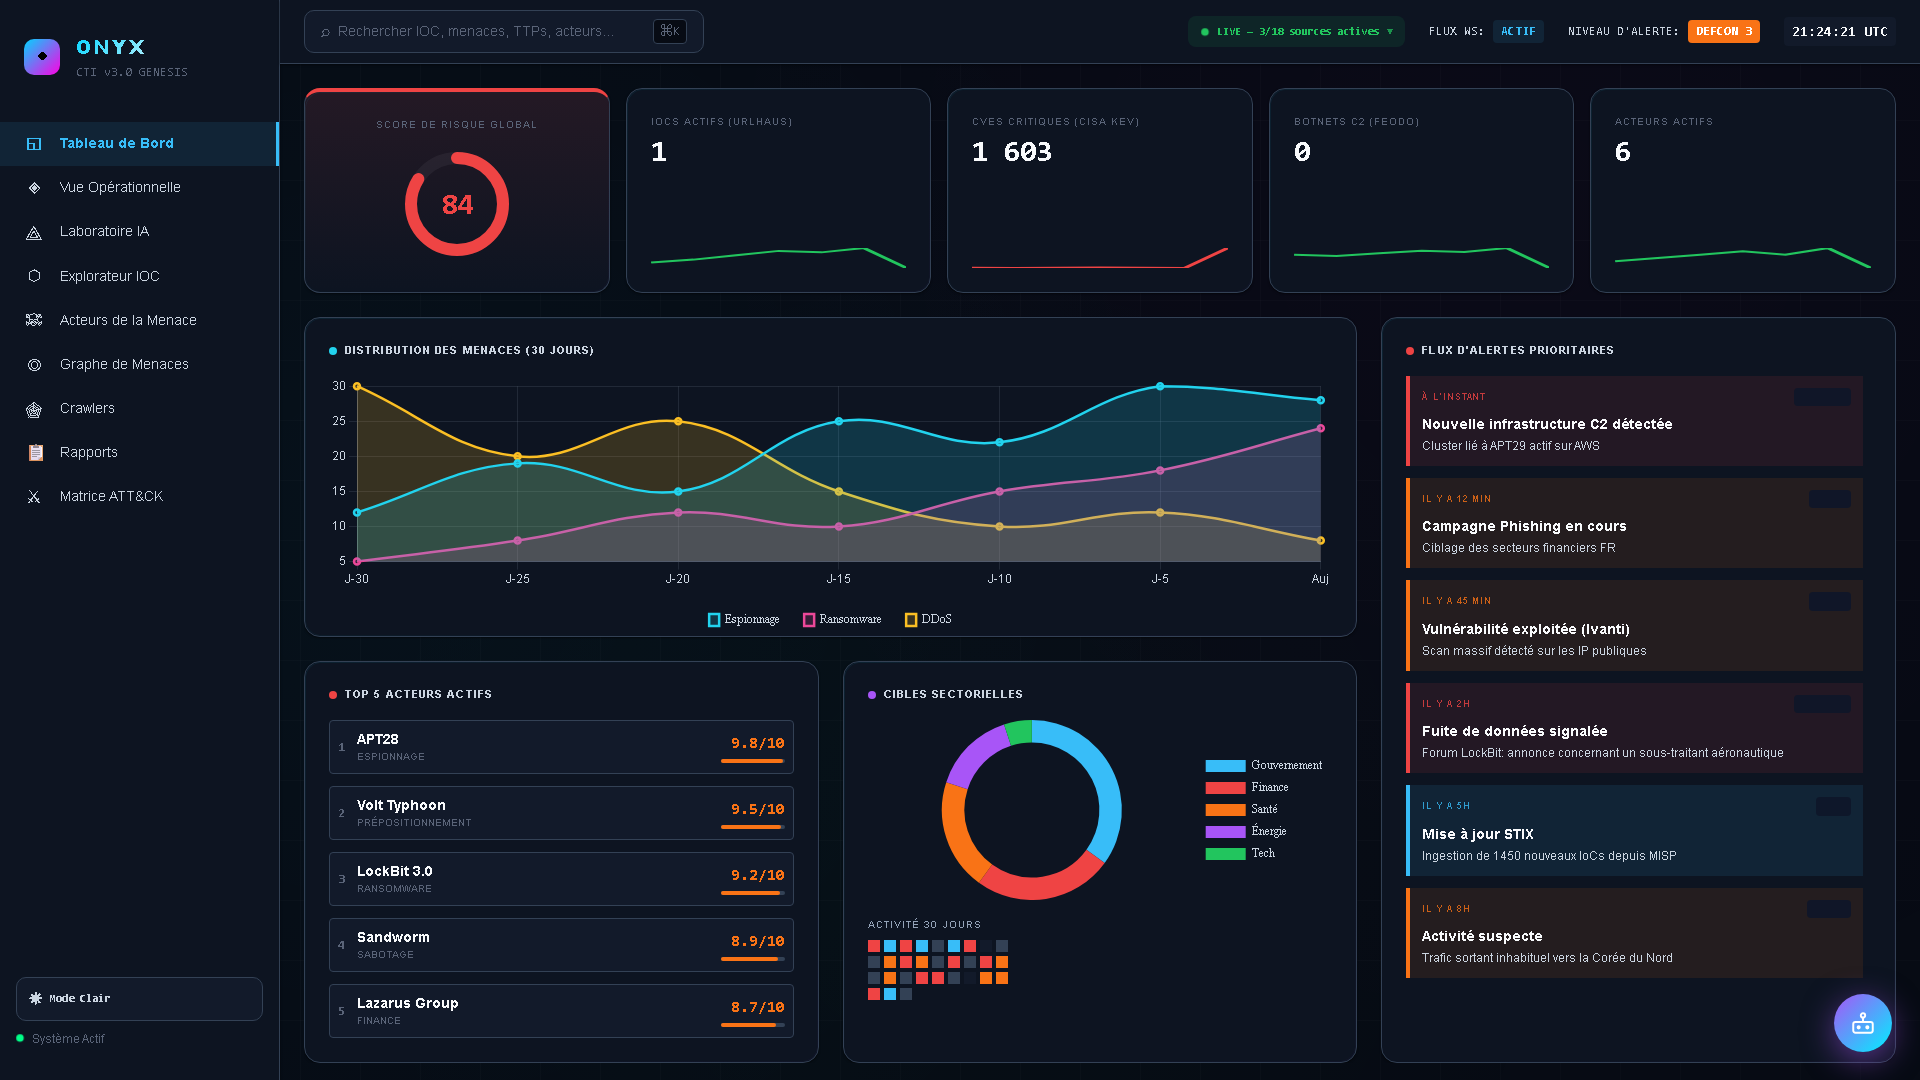
\includegraphics[width=1.0\textwidth, keepaspectratio]{dashboard_principal.png}}
    \caption{Tableau de bord principal : Agrégation en temps réel des métriques d'acquisition et des alertes CTI.}
    \label{fig:dashboard_principal}
\end{figure}

Nous observons sur cette capture plusieurs éléments qui valident le fonctionnement de bout en bout de la chaîne de traitement :

\begin{itemize}
    \item \textbf{Indicateurs d'acquisition} : les compteurs affichés (IOC armés, menaces corrélées, objets STIX) reflètent directement les sorties des pipelines d'ingestion multi-sources décrits au Chapitre~III (section~III.1). Les valeurs sont mises à jour en temps réel par le triple mécanisme d'alimentation présenté à la section précédente.
    \item \textbf{Ventilation par sévérité} : la distribution des indicateurs selon les niveaux de sévérité (critique, élevé, moyen, faible) est calculée dynamiquement à partir des scores de confiance attribués par le moteur d'extraction NLP et des métadonnées des sources OSINT. Cette distribution est cohérente avec la taxonomie de scoring définie au Chapitre~III (section~III.3.a).
    \item \textbf{État du canal WebSocket} : l'indicateur de connexion en temps réel (pastille verte et horodatage de fraîcheur) confirme l'activité du bus d'événements et la latence sous-seconde entre le serveur et le client.
    \item \textbf{Flux d'événements en direct} : les événements les plus récents, transmis par le canal WebSocket, sont affichés dans le panneau de signaux temps réel avec un code couleur correspondant à la sévérité et un horodatage précis à la seconde.
\end{itemize}

L'ensemble de ces éléments constitue une preuve fonctionnelle de l'intégration verticale de la plateforme : l'acquisition, la transformation, l'enrichissement sémantique et la restitution opèrent de manière cohérente et continue, sans intervention manuelle ni rechargement de page.
